\documentclass[
%%%%% Styles and Sizes
%10pt,
%11pt,
%12pt,
fancyheadings, % headings with seplines and logo
%
%%%%% Printing, Color and Binding
%a4paper,
%a5paper,
%twoside, % single sided printout
%oneside, % duplex printout (default)
%% binding correction is used to compensate for the paper lost during binding
%% of the document
%BCOR=0.7cm, % binding correction
%nobcorignoretitle, % do not ignore BCOR for title page
%% the following two options only concern the graphics included by the document
%% class
%grayscaletitle, % keep the title in grayscale
%grayscalebody, % keep the rest of the document in grayscale
%
%%%%% expert options: your mileage may vary
%baseclass=..., % special option to use a different document baseclass
]{stsreprt}

\usepackage{algorithm}
\usepackage{algpseudocodex}
\usepackage{amssymb}
\usepackage{biblatex}
\usepackage{booktabs}
\usepackage{csquotes}
\usepackage{mathtools}
\usepackage{microtype}
\usepackage{siunitx}
\usepackage{subcaption}
\usepackage{tikz}
\usepackage{hyperref}
\usepackage[capitalise, noabbrev]{cleveref}

\addbibresource{refs.bib}

\usetikzlibrary{graphs,graphdrawing}
\usegdlibrary{trees}

% Common Grapple algorithm math procedures
\DeclareMathOperator{\markVisited}{\texttt{mark\_visited}}
\DeclareMathOperator{\qEmpty}{\texttt{queue\_empty}}
\DeclareMathOperator{\qPop}{\texttt{queue\_pop}}
\DeclareMathOperator{\qPush}{\texttt{queue\_push}}
\DeclareMathOperator{\sSuccessor}{\texttt{state\_successor}}
\DeclareMathOperator{\sViolates}{\texttt{state\_violates}}

% Model definition math procedures
\DeclareMathOperator{\branchFreeTernary}{\texttt{BranchFreeTernary}}

% Bitstate hashing math procedures
\DeclareMathOperator{\makeHash}{\texttt{make\_hash}}

% Inline citation, e.g. "Foobar" by J. Doe [27]
\newcommand{\citeinline}[1]{\citetitle{#1} by \citeauthor*{#1} \cite{#1}}

% Biwise operators
\newcommand{\bitwiseAnd}{\mathbin{\text{\&}}}
\newcommand{\bitwiseOr}{\mathbin{\text{|}}}

% Information for the Titlepage
\author{Leonard Techel}
\title{Low-Connectivity State Space Exploration using Swarm Model Checking on the GPU}
\date{\today}
\subject{Bachelor Thesis}
\professor{Prof. Dr. Sibylle Schupp}
\advisor{Sascha Lehmann}

\begin{document}

\frontmatter

\maketitle

\chapter*{\centering \begin{normalsize}Abstract\end{normalsize}}
\begin{quotation}
    % 1. Motivation / Topic of the research area
    Using small, independent verification tests, model checking large models with billions of states can be parallelized on GPUs.
    % 2. Specific problem
    This approach works great on models with high connectivity.
    However, it fails when a model has only few edges between states or large portions of the state space are hidden behind bottleneck structures.

    % 3. Standard solutions and their limitations
    Past work on the \emph{Grapple} model checker has tried different approaches including depth-limiting and alternating between breadth-first and depth-first search.

    % 4. Outline of the new solution
    The main goal of this thesis is to:
    (1) create a systematic way of classifying a model as \emph{low-connectivity}
    (2) minimize the amount of verification tests needed to maximize the state space coverage of said models.
    To do that, we provide an implementation of the \emph{Grapple} model checker.

    % 5. How the solution was evaluated and what its outcomes are
\end{quotation}

\tableofcontents
\listofalgorithms
\listoffigures

\mainmatter

\chapter{Introduction}

% 1. Motivation / Topic of the research area

In an explicit-state model checker, state space exploration of large models with billions of states is a time-consuming problem.

Using swarm verification, the problem can be split into small, independent verification tests.
Past work has shown that by executing these verification tests in parallel on GPUs, a high-speed model checker can be implemented \cite{DeFrancisco2020.Grapple}.

GPUs are interesting for model checking because they allow a significant performance increase on parallel algorithms, are widely available and relatively cheap in comparison to specialized hardware like FPGAs/ASICs.

% 2. Specific problem

To create the small, independent verification tests, diversification is used.
Each verification test only covers a subset of the state space.
Together, the verification tests nearly achieve full state space coverage.
This approach works great on models with high connectivity.
However, it fails when a model has only few edges between states or large portions of the state space are hidden behind bottleneck structures.

\chapter{Related Work}

\begin{itemize}
    \item Parallel Breadth-First Search (BFS) \cite{Holzmann2012.Paralellizing-SPIN}
    \item Swarm Verification \cite{Holzmann2008.Swarm-Verification}
    \item Swarm Verification Techniques \cite{Holzmann2011.Swarm-Verification-Techniques}
    \item Grapple Framework \cite{DeFrancisco2020.Grapple}
    \item On-The-Fly State Generation on the GPU \cite{Bartocci2014.GPGPU-Parallel-SPIN}
\end{itemize}

\chapter{Background}

This chapter gives a brief summary on the main topics that this thesis is based on.
First, we define the scope of model checking that we are looking at in \cref{section:background:model-checking}.
We continue with an overview of Swarm Verification on the GPU and the specific problem that we are going to investigate, low-connectivity state space exploration, in \cref{section:background:parallelized-model-checking}.
Last but not least, we give an introduction to the CUDA GPU programming framework in \cref{section:background:cuda}.

\section{Model Checking}
\label{section:background:model-checking}

% What is a model checker?
% TODO Why do we search for counterexamples? The answer may fit better to the properties paragraph.
% TODO Why can it be divided into three main problems and why the specific methods stated here?
Model checking is a formal verification method that checks whether a state machine satisfies a specification.
For example, the state machine of an elevator may be verified to meet the safety property of not opening the doors between floors.
To do so, a \emph{model checker} searches the state space for counterexamples, also called violations.
When a violation is found, the path of state transitions that leads to the violation is reported back.

Model checking can be divided into three main problems:
Description of models through state machines, definition of the specification through temporal logic, and algorithms that verify whether a state machine models a specification.

%% What is an explicit-state model checker?
There are two main branches of model checking:
Explicit-State Model Checking and Symbolic Model Checking.
Explicit-State Model Checking can only verify finite state machines.
In particular, the model has to have finite states, each state needs to be representable by a finite-size tuple containing its atomic propositions, and the model changes state through execution of state transitions.
To overcome these limitations and verify potentially infinite-size state machines or systems of unknown structure, Symbolic Model Checking uses the abstraction of \emph{symbols}, each representing a set of states and transitions.
Within this thesis, we are only considering explicit-state model checking.

%% What do we want to find out with a model checker? safety, reachability, liveness, ...
% TODO Connection to temporal logic? Eventually we can skip that here.
Each state in a model is labelled with atomic propositions that hold true while the state is active.
An example for such propositions are the current values of variables in a program at a given state.
In a specification, different types of properties can then be expressed onto these propositions.
Three common properties are reachability, safety and liveness:
Reachability means that an atomic proposition holds true at some state in the future.
Safety means that an atomic proposition holds true at all states in the future.
Liveness means that an atomic proposition holds true infinitely often in the future, meaning that it does not happen that the atomic proposition never holds true.
Within this thesis, we are only considering reachability and safety properties.

%% Why is model checking so time consuming?
% TODO Introduce processes in the explicit-state model checking section
% TODO Be more precise about *what* grows exponentially and *why* this is a problem
A challenge all model checking algorithms have to face is the \emph{state explosion problem}.
In an asynchronous model of $n$ processes, each consisting of $m$ states, the number of states grows exponentially by the number of processes, namely $m^n$.
This means that even for small models, it is often not possible to fit all reachable states of the system into a computer's memory.
Therefore, every model checking algorithm needs to reduce the state space in some sense.
However, even then, a non-parallel algorithm may need a lot of physical time for exhaustive verification of the state space.
In exhaustive verification, all states are visited and checked for a violation.
\cite{Clarke2018.Introduction-to-Model-Checking,Holzmann2018.Explicit-State-Model-Checking}

\section{Parallelized Model Checking}
\label{section:background:parallelized-model-checking}

% How can model checking be speed up using parallelization?
% TODO Do we need the algorithm summary?
% TODO If yes, why leave the reader with "we are going to tell later"?
The basic operation in an explicit-state model checker is a state space exploration loop, as defined in \cref{alg:fundamental-state-space-exploration}.
Model checking can be speed up by parallelizing the state space exploration, for example using a parallel breadth-first search (BFS) \cite{Holzmann2012.Paralellizing-SPIN}.

%% What challenge is solved by Swarm Verification?
A major challenge in parallelized BFS is the communication overhead between threads:
Shared memory does not allow to easily split the work onto a cluster of heterogeneous processors or the massively parallel architecture of a GPU on which thousands of threads can exist simultaneously.

\begin{algorithm}
    \caption{Fundamental State Space Exploration Loop}
    \label{alg:fundamental-state-space-exploration}
    \begin{algorithmic}
        \While{there are unvisited states}
        \State mark state as visited
        \If{state violates spec}
        \State report path to state
        \EndIf
        \EndWhile
    \end{algorithmic}
\end{algorithm}

\subsection{Swarm Verification}
\label{section:background:swarm-verification}

%% How does Swarm Verification work?
%% How does Swarm Verification differ from other approaches?
% TODO what is state space exploration?
Swarm Verification is a new approach on parallelized model checking \cite{Holzmann2008.Swarm-Verification}.
It solves the challenge of parallelizing state-space search by splitting the state space exploration into many small, independent, memory-limited tasks called \emph{Verification Tests} (VTs).
Each VT only covers a small subset of the total state space and, using \emph{diversification techniques}, uses a different search path.
By executing all VTs and collecting their results, we still achieve nearly full state space coverage.

% The trick is that we do not care about exhaustive, 100\% state space coverage:

As VTs are independent of each other, we can easily execute them on heterogeneous computers.
Even further, as VTs are also memory-limited, we can massively parallelize them on devices with very limited resources like GPUs.

%% What is diversification and which diversification techniques exist?
Multiple diversification techniques can be applied, e.g. randomizing the order of nondeterministic choice on states with multiple outgoing transitions or reversing the search order.
The most powerful diversification technique is state pruning using hash collisions:
During state exploration, states get marked as visited in a limited-size hash table.
By using a different hash function for each VT, the state space gets automatically pruned through hash collisions.
The process is illustrated in \cref{fig:hash-collision-state-pruning}, that shows an example state graph on which BFS is performed by two VTs.
On the left side, state B and C cause a hash collision, resulting in the subgraph originating in state C being removed.
On the right side, state E and F cause a hash collision, resulting in the subgraph originating in state F being removed.
Each state exploration on its own does not cover the whole state space, however, by combining the results from both searches, all states are covered again.

% TODO How to cite this? It is taken from the Grapple paper :)
\begin{figure}
    \begin{subfigure}[b]{.5\textwidth}
        \centering\resizebox{.8\textwidth}{!}{
            \begin{tikzpicture}[nodes={draw, circle}]
                \graph [tree layout, missing nodes get space] {
                    A [fill=lightgray];
                    B [fill=lightgray];
                    D [fill=lightgray];
                    E [fill=lightgray];
                    F [fill=lightgray];
                    I [fill=lightgray];
                    J [fill=lightgray];

                    A -- B [second];
                    A -- C;
                    A -- D;

                    B -- E;
                    B -- F;

                    C -- F;
                    C -- G;
                    C -- H;

                    D -- I;

                    F -- J;

                    H -- K;
                    H -- L;
                };
            \end{tikzpicture}
        }
        \subcaption*{Collision: \{B, C\}}
    \end{subfigure}
    \begin{subfigure}[b]{.5\textwidth}
        \centering\resizebox{.8\textwidth}{!}{
            \begin{tikzpicture}[nodes={draw, circle}]
                \graph [tree layout, missing nodes get space] {
                    A [fill=lightgray];
                    B [fill=lightgray];
                    C [fill=lightgray];
                    D [fill=lightgray];
                    E [fill=lightgray];
                    G [fill=lightgray];
                    H [fill=lightgray];
                    I [fill=lightgray];
                    K [fill=lightgray];
                    L [fill=lightgray];

                    A -- B;
                    A -- C;
                    A -- D;

                    B -- E;
                    B -- F;

                    C -- F;
                    C -- G;
                    C -- H;

                    D -- I;

                    F -- J;

                    H -- K;
                    H -- L;
                };
            \end{tikzpicture}
        }
        \subcaption*{Collision: \{E, F\}}
    \end{subfigure}
    \caption{State pruning using hash collisions}
    \label{fig:hash-collision-state-pruning}
\end{figure}

\subsection{Grapple Framework}

% What is Grapple?
The paper \citeinline{DeFrancisco2020.Grapple} which this thesis is based on contributes the \emph{Grapple} framework for parallel swarm verification on the GPU using CUDA.
In their implementation of Swarm Verification, each VT's state space exploration runs in a parallel BFS, using CUDA's built-in synchronization primitives to coordinate threads.

%% Which variations of the algorithm exist?
%% How does the Grapple algorithm work?
%% How can the Grapple algorithm and its in- and outputs be formally defined?

\subsection {Low-Connectivity Models}

% What are Low-Connectivity models?
A key observation of \cite{DeFrancisco2020.Grapple} is that their algorithm's state space coverage in relation to the number of executed VTs slows down on models with \emph{low connectivity}.
A model has \emph{low connectivity} if at least one of the following properties is satisfied:

\begin{itemize}
    \item \textbf{Generally Linear}: The average number of edges per state is close to two: One inbound, one outbound
    \item \textbf{Bottleneck Structures}: A single state or group of states other than the initial state that needs to be passed to reach most of the state space
\end{itemize}

See \cref{fig:lc-ex} for examples of these properties.

%% How can a model be classified as Low-Connectivity? (technically vs. theoretically ?)
%% Why is the Grapple search algorithm so slow on Low-Connectivity models?

\begin{figure}
    \begin{subfigure}[b]{.5\textwidth}
        \centering
        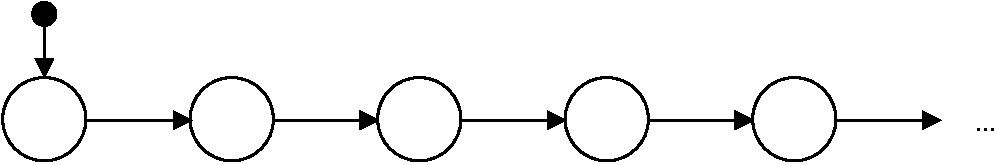
\includegraphics[width=\textwidth]{figures/lc-ex-generally-linear}
        \subcaption{Example of a generally linear graph}
        \label{fig:lc-ex-generally-linear}
    \end{subfigure}
    \begin{subfigure}[b]{.5\textwidth}
        \centering
        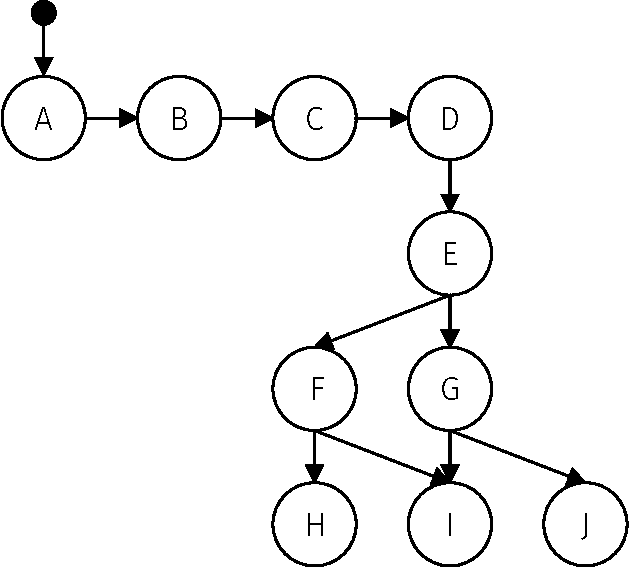
\includegraphics[width=.9\textwidth]{figures/lc-ex-bottleneck}
        \subcaption{Example of a bottleneck structure}
        \label{fig:lc-ex-bottleneck}
    \end{subfigure}
    \caption{Examples of low-connectivity properties}
    \label{fig:lc-ex}
\end{figure}

\section{CUDA}
\label{section:background:cuda}

% How can many small tasks be executed in parallel? What is CUDA?
%% What challenge does CUDA solve?
CUDA is NVIDIA's proprietary GPU programming framework that provides automatic massive scalability.

%% What is the abstraction model of CUDA?
The CUDA model defines a three-level abstraction.
At the lowest level, a program function called \emph{kernel} is defined using C/C++.
The kernel is executed by defining the amount of \emph{threads} and \emph{blocks} that run in a \emph{grid}:
Each grid contains multiple blocks.
Each block contains multiple threads.
Each thread in a block executes the kernel function using the single instruction, multiple thread (SIMT) execution model.
Thus, each thread should work on an independent piece of memory.
Only threads within a block can cooperate, for example using shared memory or synchronization barriers.

Internally, the GPU, also called \emph{device}, maps the blocks of threads onto its \emph{streaming multiprocessors}.
By doing so, tens of thousands of threads can be executed in parallel.
The architecture allows scaling even further onto multiple GPUs.

Furthermore, CUDA defines multiple memory levels, each with different size and access speed.
% CUDA Toolkit v11.4.1, Programming Guide, Table 15

\begin{itemize}
    \item \emph{Registers} are used for thread-local variables.
          There can be at max 255 registers à 32 bit per thread.

          % \item \emph{Local memory}

    \item \emph{Shared memory} can only be accessed by the threads of the block in which it got allocated.
          As it is on-chip, it is faster than global memory.
          By default, there is 48 KB of shared memory.

    \item \emph{Constant memory} is part of the device memory, with the constant cache in front of it.
          Cache hits are served at higher speed than just using global memory.
          There is 64 KB of constant memory.

          % \item \emph{Texture cache}

    \item \emph{Global memory} is the largest memory with usually multiple gigabytes of size.
          It is placed in device memory and thus also the slowest.
\end{itemize}

%% Why are GPUs so interesting for swarm verification / model checking?
CUDA requires the problem to be solved by a program to be split into many small sub-problems.
This is a good fit with Swarm Verification, which turns the model checking problem into many small, independent VTs.

% - Challenge: Where to parallelize?

% TODO Graphic of the CUDA architecture
% TODO Example CUDA kernel, as in the intermediate presentation

\chapter{Theory}
\label{chapter:theory}

This chapter gives a detailed explanation of the algorithms used by our model checker.
It starts with an in-depth description of the Grapple framework's state space exploration loop and its components in \cref{section:theory:grapple-model-checker}
We then continue with a list of known state space diversification techniques in \cref{section:theory:state-space-diversification}.
The chapter finishes with a solution to the problem of counting the number of unique states visited in Swarm Verification in \cref{section:theory:counting-unique-states-visited}.

% TODO what about the theory behind low-conn models ?

\section{Model Definition}
\label{section:theory:model-definition}

%% How are Models defined?
The model is defined using a \emph{Kripke Structure} $M = \left(S; S_0; R; L \right)$ where $S$ is the finite set of states, $S_0 \in S$ is the finite set of initial states $S_0 \subseteq S$, $R \subseteq S \times S$ is the left-total transition relation and $L : S \mapsto 2^{AP}$ is the labelling function that assigns each state its atomic propositions.

%% How are properties defined? (temporal logic)

\section{Grapple Model Checker}
\label{section:theory:grapple-model-checker}

% How can the verification tests be run on GPUs using CUDA?
In Grapple, each VT executes an internally parallel state space exploration.
We call it \emph{internally parallel} to differentiate between the parallelism \emph{within} a VT and the parallelism \emph{between} multiple VTs.

Each thread in a VT executes \cref{alg:grapple-state-space-exploration}, which is a more abstract version of the Grapple state space exploration loop (Algorithm 1 in \cite{DeFrancisco2020.Grapple}).
We are going to call this algorithm the \emph{Grapple algorithm}.
The Grapple algorithm is based on Holzmann's parallel BFS \cite{Holzmann2012.Paralellizing-SPIN}.

% TODO is this still true? i think no
% We currently only support a single initial state.

\subsection{Model Definition and State Generation}
\label{section:theory:model-definition-state-generation}

%% What is the difference between on-the-fly and a priori state generation?
State generation strategies of model checkers can be divided into \emph{a priori} and \emph{on-the-fly} generation.
In a priori generation, the state space graph is completely known before running the verification algorithm, for example as an adjacency matrix.
In on-the-fly generation, the successors of each state are created on the fly during verification.
Grapple uses on-the-fly generation on the GPU.
Furthermore, Grapple can only verify models with the same number of nondeterministic choices

\[M = \left(\left(S; S_0; R; L\right); P; \mathit{NDC}\right)\]

%% Which operations does the model have?
The states of a model support two operations: $\sSuccessor(p, ndc, state)$ on-the-fly returns a successor to a state and $\sViolates(state)$ returns whether a state violates.

\begin{align*}
    \sSuccessor
    : S \times \mathit{NDC} \times \mathit{P}
    \mapsto S
\end{align*}

\begin{align*}
    \sViolates
    : S
    \mapsto \left\{0, 1\right\}
\end{align*}

\subsection{Queues}
\label{section:theory:queues}

%% What is the purpose of the queues?
In summary, the parallel BFS is implemented using lock-free communication between threads via a shared, multidimensional queue array.
Being lock-free removes the overhead of waiting for locks to be released and allows the algorithm to be split up onto many threads, limited only by the quadratic queue size.

%% How do the queues work?
For each pair of threads, there is only one piece of memory to communicate over.
Writing and reading to this piece of memory is coordinated by splitting the algorithm into two alternating phases:

In the first phase $t=0$, each thread $i$ processes all states from its input queues $Q\left[t\right]\left[ 0 \dots N \right]\left[i\right]$.
Here, $N$ denotes the amount of threads executing a VT, with $N=32$ being the default.
For each input state, successors are generated on-the-fly.
For each successor, we check whether it is already visited in a hash table.
If a successor is priorly unvisited, we check whether it violates.
Violating successors are reported to the host using a buffer.
Non-violating successors are written to a random worker $j$'s input queue $Q\left[1 - t\right]\left[i\right]\left[j\right]$.
When all input states are processed and threads are synchronized, the phases get swapped, i.e. $t = 1 - t$.
This process repeats until no more unvisited successors are discovered.

% TODO explain why we have a multi-slot queue for each thread ???

%% Which operations does the queues have?
The queues support three operations: $\qPush(Q, state)$ adds a state to the back, $\qPop(Q)$ removes and returns the first state from the front and $\qEmpty(Q)$ tells whether a queue is empty.

\subsection{Hash Table}
\label{section:theory:hash-table}

%% Which operations do the hash tables have?
The hash tables support one operation: $\markVisited(V, state)$ marks a state as visited and returns whether it was already visited before.

%% How do the bit state hash table work and how can we control the collisions?


% TODO Validity: For which inputs does the algorithm work?
% \paragraph{Validity}

% TODO Correctness: Are all criteria fulfilled? Ex: Is every discovered violation actually a violation?
% \paragraph{Correctness}

% Completeness: Does the algorithm find all violations?
\paragraph{Completeness} A big challenge in Swarm Verification is the question on how much of the state space is actually covered, i.e. whether all violations are found.
Due to overlap in state space between VTs and the sheer amount of states being checked by each VT, computing the exact number of unique states visited and thus the exact state space coverage can hardly be done.
Instead, we can estimate the state space coverage, as described in \cref{section:theory:counting-unique-states-visited}.

% Termination: When/Does/Under which (input) conditions does the algorithm terminate?
\paragraph{Termination}
The algorithm terminates when there are no more unvisited state successors according to the hash table.
In this case, all input queues of the next phase remain empty, i.e. $Q\left[1 - t\right]\left[0 \dots N\right]\left[0 \dots N\right] = \emptyset$.

There are two reasons why at some point no more unvisited states get discovered:
Either, we did an exhaustive verification of the model, meaning that all states actually got visited.
Or, which happens most of the time in Grapple, the hash table is full, causing a collision of every new successor with an already visited state.
Collisions are intended, as mentioned in \cref{section:background:swarm-verification}.

Resulting from this, the algorithm at worst terminates after having visited the number of states being the minimum of queue size and state space size.

\begin{algorithm}
    \caption{Grapple state space exploration loop of a single worker}
    \label{alg:grapple-state-space-exploration}
    \begin{algorithmic}
        \State $t \in \left\{0, 1\right\} \gets 0$
        \Comment{Current algorithm phase}
        \State $\mathit{visited} \subseteq S \gets \emptyset$
        \Comment{Hash table of visited states}
        \State $Q[2][N][N][I] \gets \emptyset$
        \Comment{Queues}
        \Statex
        \LComment{Initial state}
        \State $\qPush(Q[t][0][0], S_0[0])$
        \State $\markVisited(S_0[0])$
        \Statex
        \State \texttt{\_\_syncthreads()}
        \Statex
        \State $done \gets \text{false}$
        \While{not $done$}
        \For{$i = 0, \dots, N$}
        \While{not $\qEmpty(Q[t][\text{threadIdx.x}][i])$}
        \State $state \gets \qPop(Q[t][\text{threadIdx.x}][i])$
        \For{$p \in \text{processes}$}
        \For{$\mathit{ndc} \in \text{nondeterministic choices within } p$}
        \State $succ \gets \sSuccessor(p, ndc, state)$
        \State $visited \gets \markVisited(succ)$
        \If{not $visited$}
        \If{$\sViolates(succ)$}
        \State report path to state
        \Else
        \State $next \gets \text{random output queue } n \in N$
        \State $\qPush(Q[1 - t][next][\text{threadIdx.x}], succ)$
        \EndIf
        \EndIf
        \EndFor
        \EndFor
        \EndWhile
        \EndFor
        \Statex
        \State \texttt{\_\_syncthreads()}
        \Statex
        \State $done \gets \qEmpty(Q[1 - t][0 \dots N][\text{threadIdx.x}])$
        \State $t \gets 1 - t$
        \Statex
        \State \texttt{\_\_syncthreads()}
        \Statex
        \EndWhile
    \end{algorithmic}
\end{algorithm}

\section{State Space Diversification}
\label{section:theory:state-space-diversification}

% TODO Section introduction
% TODO Difference between graph partitioning and state space diversification?

\subsection{Diversification Techniques}

The following diversification techniques are known: \cite{Holzmann2011.Swarm-Verification-Techniques,DeFrancisco2020.Grapple}

\begin{itemize}
    \item \textsf{State Pruning using Hash Collisions} \\
          Each VT marks its visited states in a limited-size hash table, each using a different hash function.
          Hash collisions cause different partitions of the state space.
          Hash table exhaustion causes termination of the exploration when all new states are supposedly already visited.
    \item \textsf{Reverse order of nondeterministic choice} \\
          Iterate through nondeterministic choices in reverse order, i.e. $\mathit{NDC}{\dots}0$.
    \item \textsf{Reverse processes} \\
          Iterate through processes in reverse order, i.e. $P{\dots}0$.
    \item \textsf{Random order of nondeterministic choice} \\
          Instead of iterating through nondeterministic choices from $0{\dots}\mathit{NDC}$, choosing one random order for each VT.
          The random order remains the same through all searches in a VT.
    \item \textsf{Random process order} \\
          Instead of iterating through processes from $0{\dots}P$, choosing one random order for each VT.
          The random order remains the same through all searches in a VT.
    \item \textsf{Parallel Deep Search (PDS)} \\
          Select one random nondeterministic choice per VT, discard others.
          The selected nondeterministic choice remains the same through all searches in a VT.
    \item \textsf{process-PDS} \\
          Select one random process per VT, discard others.
          The selected process remains the same through all searches in a VT.
\end{itemize}

\subsection{State Pruning and Start Overs}
\label{section:theory:state-pruning}

% How are partitions made with State Pruning using Hash Collisions?


% Why do we need to lower the hash table's size? What problem arises from this?
% How does starting over solve the problem of a lowered hash table size?
% How does starting over solve the problem of deep exploration?

\section{Waypoints Model}
\label{section:theory:waypoints-model}

% Where does the WP model come from? What is it good for? (benchmark)
The Waypoints (WP) model is a benchmark for Swarm Verification model checkers.
It is first introduced in \cite{Holzmann2011.Swarm-Verification-Techniques} and is used as primary benchmark in \cite{DeFrancisco2020.Grapple}.
Our implementation is defined in \cref{alg:waypoints-model}.

% How does the state machine of the WP model work?
The model creates a state space of the size of all 32-bit integers, i.e. $2^{32}=\num{4294967296}$ states.
To do so, it uses eight processes, each in control of four bits.
At successor generation, each process will nondeterministically set one of its bits.

% What properties are verified on the WP model?
There is a single reachability property:
We predefine a set of 100 uniform randomly chosen 32-bit integers, called \emph{waypoints}.
A state violates if it is part of the set.
As the waypoints are uniformly distributed, the number of unique discovered waypoints is equal to the percentage of state space coverage.
For example, 24 discovered waypoints means that approximately $24\%$ of the state space is covered.

\begin{algorithm}
    \caption{Waypoints model}
    \label{alg:waypoints-model}
    \begin{algorithmic}
        \State $violations \gets \left\{\text{100 random 32-bit integers}\right\}$

        \Statex

        \Function{$\sSuccessor$}{$p$, $ndc$, $state$}
        \State \Return $state \bitwiseOr 1 << ((4 \cdot process) + ndc)$
        \EndFunction

        \Statex

        \Function{$\sViolates$}{$state$}
        \State \Return $state \in violations$
        \EndFunction
    \end{algorithmic}
\end{algorithm}

\section{Low-Connectivity Models}

% What is the challenge in exploring LC models using the presented algorithm?


\section{Counting Unique States Visited}
\label{section:theory:counting-unique-states-visited}

% Why do we need to count unique states visited?
In Swarm Verification, we achieve a much faster verification by only covering \emph{nearly} 100\% of the state space.
Resulting from this, it is important to know how much of the state space is actually covered.
To find this out, we need to count unique states visited.

% Where does the total number of states of a model come from?
To calculate the percentage of state space covered, we have to know the total state space size.
As in this thesis we only consider models with known state space size, we can provide it as pre-calculated constant.

% Why can we only estimate the amount of unique states visited?
The executed VTs may overlap in explored state space, meaning that across all VTs, a state may be visited multiple times.
In order to calculate the exact number of unique states visited, we have to identify distinct states in the stream of all visited states.
This is called the \emph{count-distinct problem}.

Intuitively, one could collect all visited states in a set and then take its cardinality.
However, this approach requires an amount of memory proportional to the amount of visited states which, as of the state space explosion problem, results in exponential memory usage.

A solution to this problem are \emph{probabilistic cardinality estimators} that approximate the number of unique states within a fixed error using significantly less memory.

% How can HyperLogLog be used to do the counting?
We choose the algorithm introduced in \citeinline{Flajolet2007.HyperLogLog}, as it is commonly used and relatively easy to implement.

For each VT, we create a HyperLogLog.
Inside each VTs state space exploration, we call the \texttt{add} operation for each newly discovered state.
When a VT has finished, we \texttt{merge} its HyperLogLog with those of all other already finished VTs.
We then can execute the \texttt{estimate} operation on the global HyperLogLog to get the estimation of unique visited states across all finished VTs.

% Where does HyperLogLog fail? What can we do about it?
% TODO Move this section to implementation / evaluation ?
Cardinality estimation with HyperLogLog yields good results on the Dining Philosophers problem with 15 processes and $3^{15}-1$ states.
As expected, the number of unique states visited grows logarithmic until reaching around 100\%.
However, on the Waypoints model with $2^{32}$ states, the estimation fails.

The paper \citeinline{Heule2013.HyperLogLog++} finds out that the estimation of cardinalities beyond one billion fails on the original HyperLogLog algorithm.
They solve this problem by using a 64-bit hash instead, calling their improved algorithm HLL++.

% TODO Can we fix our problem by using HLL++? - YES
Using HLL++, we can count unique states visited.

\chapter{Implementation}

% What is the goal of our implementation?
Our implementation serves two purposes:
To reproduce the results from the Grapple paper \cite{DeFrancisco2020.Grapple}.
And to run our experiment series on the state space exploration of low-connectivity models.

% What is the content of this chapter?
This chapter documents our implementation of a Grapple model checker.
The general architecture of the model checker is described in \cref{section:implementation:source-code}.
Usage instructions are described in \cref{section:implementation:usage}.

\section{Source code}
\label{section:implementation:source-code}

% What programming language, build tools, frameworks, ... are used?
We chose C++17 as programming language, so we can make full use of the CUDA Toolkit, which is provided as C header.
The CUDA Toolkit is used in version 11.4.
As build system, CMake 3.16 is used.
Code is written using the Object-Oriented Programming paradigm.
%% Of which components does the Grapple model checker consist?
Our implementation consists of six components:

\begin{enumerate}
    \item The main program, running the CUDA kernels and collecting their results.
    \item The CUDA kernel, implementing a parallel state space exploration loop.
    \item The queues, providing lock-free communication between threads in a VT.
    \item The hash tables in which states are marked as visited.
    \item The model, providing successor generation and violation checking.
    \item The HyperLogLog, counting unique states visited across all VTs.
\end{enumerate}

% TODO visualize the architecture

In the following, we are going to describe the implementation-specific details and challenges of each component.

\subsection{Main Program}

% What does the main program do?
The main program runs in a single thread on the host.
On startup, it seeds a global pseudorandom number generator (PRNG) and creates a random value for each CUDA thread.
Then, for each run, it executes the CUDA kernel in a grid of $K=250$ blocks, each consisting of $N=32$ threads.
% How is the algorithm mapped onto the CUDA architecture?
Each block represents a VT, meaning that VTs are executed in batches of 250.
Each thread represents a worker of a VT's parallel state space exploration.
% How do we post-process output data of the kernels?
After each run, the main program collects the discovered violations and number of unique states visited, accumulates them and prints them to the standard output line-by-line as CSV.

\subsection{CUDA Kernel}

% What does the Grapple CUDA kernel do?
The CUDA kernel executes the state space exploration loop, as described in \cref{section:theory:grapple-model-checker}.

%% How can the variations (PDS, process-PDS, scatter-PDS, ...) be implemented?

\subsection{Queues}

% How are the queues implemented?
The queues provide a data structure for lock-free communication between threads in a VT, as described in \cref{section:theory:queues}.
By default, each queue has a capacity of $I=4$ states.
They are only used on-device within the CUDA kernel and stored in global memory due to the limited size of shared memory.
Resulting from this, we have to map $K \times 2 \times N \times N \times I$ queues into memory.
This proposes two challenges:
1. We have to implement fixed-capacity queues.
2. We have to map multidimensional queues into a one-dimensional, linear memory allocation.

% How are the fixed-capacity queues implemented?
% TODO describe push and pop using pseudocode?
Usually, fixed-capacity queues are implemented as ring buffer.
However, due to the design of the two-phase parallel state space exploration, it is sufficient to implement the queue as a singly linked list.
In addition to that, we have to keep a pointer to the \texttt{head} and \texttt{tail} of the linked list.
Then, in the first phase, each queue is filled through the $\qPush$ operation by adding an element to its linked list and updating the \texttt{tail}, until the \texttt{tail} points to the last element in memory.
In the second phase, each queue is completely emptied through the $\qPop$ operation by retrieving the \texttt{head}, then incrementing it until \texttt{head} equals \texttt{tail}.
A queue is empty if both \texttt{head} and \texttt{tail} are null pointers.

% How are the multidimensional queues mapped into memory?
The memory address of thread $i$'s input queue, which is an output queue of thread $j$, in algorithm phase $t$, of VT $v$, is calculated using the formula:
\[v \cdot (2 \cdot N \cdot N) + t \cdot (N \cdot N) + j \cdot N + i\]

\cref{fig:4d-mapped-memory} illustrates the mapping of a single example VT with $K=1$ and $N=4$, meaning that we allocate memory for $1 \times 2 \times 4 \times 4 = 32$ queues.
On the top row, each slot represents the memory allocation of a single queue.
The remaining rows illustrate the constants enclosed in parentheses in our formula:
Each set of output queues has a width of $N$, which we have to multiply with the index of the current thread to get at its first memory slot.
Each phase has a width of $(N \cdot N)$, which we have to multiply with the index of the current phase.
Each VT has a width of $(2 \cdot N \cdot N)$, which we again have to multiply with the index of the current VT to get to its first memory position.
By adding up all products, and adding the index of the current input queue, we get the address of the exact slot.

% TODO better graphic using curly braces instead of boxes
\begin{figure}[h]
    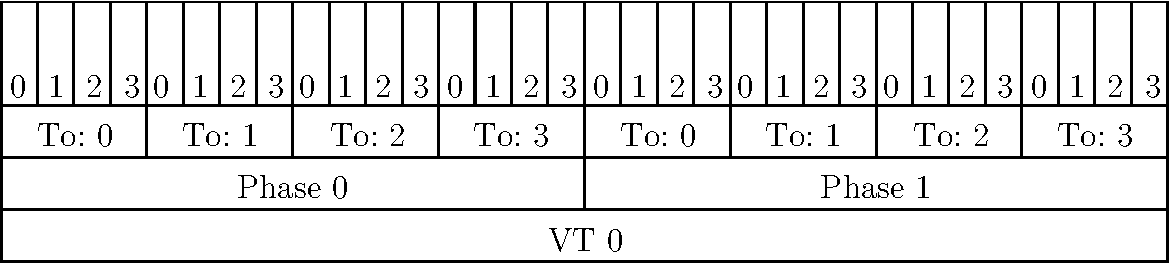
\includegraphics[width=\textwidth]{figures/4d-mapped-memory}
    \caption{A single VT of the 4D array, mapped to 1D memory}
    \label{fig:4d-mapped-memory}
\end{figure}

\subsection{Model and Successor Generation}

% How are models implemented?
Models are implemented using a data structure that represents a current state.
Each state instance then provides the two operations $\sSuccessor$ and $\sViolates$.
The state instances are stored in the queues.

%% How can states be created on-the-fly on the GPU?
State generation is usually heavily based on branching through \texttt{switch}- and \texttt{if}-conditions.
However, CUDA's SIMT execution model, in which warps of 32 threads operate on same instruction, causes threads to pause when their execution paths diverge.
This means that state generation through branching results in a slower CUDA execution.
As a countermeasure, \citeauthor*{Bartocci2014.GPGPU-Parallel-SPIN} propose to calculate all possible state transitions every time, preserving the SIMT execution and at the same time creating different states in each thread \cite[Algorithm 3]{Bartocci2014.GPGPU-Parallel-SPIN}.
To do so, it makes use of the custom ternary operator described in \cref{alg:branching-free-ternary-operator} that exploits the fact that boolean values evaluate to either zero or one.

\begin{algorithm}
    \caption{Branching-Free Ternary Operator}
    \label{alg:branching-free-ternary-operator}
    \begin{algorithmic}
        \Function{$\branchFreeTernary$}{bool c, int t, int f}
        \State \Return $c \cdot t + (1 - c) \cdot f$
        \EndFunction
    \end{algorithmic}
\end{algorithm}

A key difference of our implementation is that we do not fit a state's variables into a single integer using bit shifts.
Instead, we use regular C++ class data members.
The increased memory demand by regular data members can be neglected, as the queues in which we store state instances are in global memory which is usually gigabytes in size.
Also, the same behavior as in the paper can be achieved using C++ bit field members.

Using our custom ternary, we can re-use DVE models from the discontinued BEEM model database\footnote{\url{https://paradise.fi.muni.cz/beem/}}.
DVE is a file format used by the DIVINE 3 model checker.
We translate DVE models into CUDA compatible C++ with the template described in \cref{alg:on-the-fly-state-generation-on-the-gpu}.

% TODO explain the on-the-fly GPU state generation algorithm

\begin{algorithm}
    \caption{On-The-Fly State Generation on the GPU}
    \label{alg:on-the-fly-state-generation-on-the-gpu}
    \begin{algorithmic}
        \LComment{Global variables}
        \State $glob \gets 0$
        \LComment{Process-Local variables use arrays. Here, N is the number of processes}
        \State $state[N] \gets \{0, \dots, 0\}$

        \Statex

        \Function{$\sSuccessor$}{p, ndc, state}
        \LComment{Evaluate all guards before calculating transitions}
        \State $guard_1 \gets state[p] = 0$
        \State $guard_2 \gets state[p] = 1 \land glob \leq 2$
        \State $guard_3 \gets state[p] = 1 \land glob > 2$

        \LComment{Transition from state 0 to 1}
        \State $next.state \gets \branchFreeTernary(guard_1, 1, state.state)$

        \LComment{Transition from state 1 to 1}
        \State $next.glob \gets \branchFreeTernary(guard_2, state.glob + 1, state.glob)$
        \State $next.state \gets \branchFreeTernary(guard_2, 1, next.state)$

        \LComment{Transition from state 1 to 0}
        \State $next.glob \gets \branchFreeTernary(guard_3, 0, next.glob)$
        \State $next.state \gets \branchFreeTernary(guard_3, 0, next.state)$

        \Statex

        \State \Return $next$
        \EndFunction
    \end{algorithmic}
\end{algorithm}

% https://docs.nvidia.com/cuda/cuda-c-programming-guide/index.html#simt-architecture
% https://docs.nvidia.com/cuda/cuda-c-programming-guide/index.html#control-flow-instructions

\subsection{Hash Tables}
\label{section:implementation:hash-tables}

The hash tables provide a data structure in which states are marked as visited.
They are only used on-device within the CUDA kernel and stored in shared memory, resulting in a highly constrained size.
Each VT operates on a single hash table, meaning that all threads in a block share one hash table.
For memory efficiency, we use bitstate hashing \cite{DeFrancisco2020.Grapple}.
Our hash tables can store $2^{18}=\num{262144}$ states, taking up \num{32768} bytes of shared memory.

% How does bitstate hashing work?
In bitstate hashing, a single bit represents whether a state is visited.
Per clock cycle, CUDA can transmit 32 bit of shared memory, which is stored in 32-bit words.
Resulting from this, we use a bucket size of 32 bit.
The bit representing whether a state is visited is then computed using \cref{alg:bitstate-hashing}.

% How can we control collisions?
The hash function's goal is to map random data with unknown distribution onto a nearly uniform distribution, so each bucket of the hash table is used equally likely.
In our implementation, hashing is done using the Jenkins Hash function\footnote{\url{https://www.burtleburtle.net/bob/hash/doobs.html}}.
The MurMurHash3\footnote{\url{https://github.com/aappleby/smhasher}}, which is used by our HyperLogLog, yields similar results.

Hash collisions resulting in false-positives are intended, as explained in \cref{section:theory:state-pruning}.
To achieve that in every VT different states cause a collision, each is including a different seed into the hash.
The rate of collisions can then be controlled by the hash table's size.

\begin{algorithm}
    \caption{Bitstate hashing}
    \label{alg:bitstate-hashing}
    \begin{algorithmic}
        \LComment{Initialize hash table buckets. Here, $N$ is the hash table size}
        \State $table[(1 << N - 5)] \gets \{0, \dots, 0\}$

        \Statex

        \Function{$\markVisited$}{state}
        \State $hash \gets \makeHash(state, seed) \bitwiseAnd (1 << N) - 1$

        \LComment{First 5 bits ($2^5=32$) are the index within the bucket}
        \State $elem \gets hash >> (N - 5)$

        \LComment{Last $N-5$ bits are the bucket index}
        \State $bucket \gets hash \bitwiseAnd (1 << N - 5) - 1$

        \LComment{Retrieve current state}
        \State $isVisited \gets table[bucket] \bitwiseAnd (1 << elem) \neq 0$

        \LComment{Update hash bucket}
        \State $table[bucket] \gets table[bucket] \bitwiseOr (1 << elem)$

        \Statex

        \State \Return $isVisited$
        \EndFunction
    \end{algorithmic}
\end{algorithm}

\subsection{HyperLogLog++}

The HyperLogLog (HLL) provides an algorithm for distributed counting of distinct elements, as described in \cref{section:theory:counting-unique-states-visited}.
In our implementation, the grid of VTs of each run is operating on a single HLL that is stored in global memory.
Visited states are added to the HLL only on-device.
The host collects the HLLs after the kernels have finished, merge them into one big HLL and does the estimation of unique states visited.
Merging and estimating the amount of unique states visited is done only on the host.

\section{Usage}
\label{section:implementation:usage}

To verify a model using our model checker, a user has to complete the following steps:

\begin{enumerate}
    \item Describe their model in a C++ class using \cref{alg:on-the-fly-state-generation-on-the-gpu}
    \item Compile our model checker including their model
    \item Execute the single output binary.
          On execution, the user may set the PRNG seed and number of runs using command-line options.
          The number of runs needed to achieve a certain state space coverage needs to be evaluated experimentally.
    \item Interpret the CSV output
\end{enumerate}

\chapter{Evaluation}

% This chapter presents empirical experimental results of our implementation.
This chapter presents our series of empirical experiments conducted on our implementation.
It starts with experiments on the correctness of our implementation and a comparison with the Grapple paper's results in \cref{section:evaluation:correctness-comparison-with-paper}.
We then continue with a series of experiments that compare the Waypoints model, which is known to be high-connectivity, with three low-connectivity models in \cref{section:evaluation:low-connectivity-model-evaluation}.

All experiments are performed on an NVIDIA GeForce RTX 2080 Ti GPU, using the randomly chosen hash seed 1736331306.

The calculation of visited state space is done using a HLL with $2^{14}$ registers.
% TODO move the following sentences into the HyperLogLog's theory section
This means that there may be a relative error of $\sigma=1.04 / \sqrt{2^{14}}=\num{0.008125}$.
The 65\% error bound for each value $x$ is then $\left[x \cdot (1-\sigma), x \cdot (1+\sigma)\right]$.
95\% and 99\% can be reached using $2\sigma$ and $3\sigma$.

\section{Correctness and Comparison with the Paper}
\label{section:evaluation:correctness-comparison-with-paper}

We start the evaluation with whether our implementation reaches the same number of discovered waypoints in relation to the amount of executed VTs as presented in the Grapple paper.
We would expect both implementation to behave similarly, discovering at least 80 waypoints in \num{20000} VTs and all 100 waypoints in about \num{100000} VTs, as shown in \cref{fig:evaluation:EXP-00:1}.
However, that is clearly not the case, as presented in \cref{fig:evaluation:EXP-00:2}.
Our implementation finds significantly fewer waypoints, even though the amount of VTs is 2.5x larger.

To further investigate differences between the implementations, we conduct additional experiments.

\begin{figure}[h]
    \begin{subfigure}[b]{.5\textwidth}
        \centering
        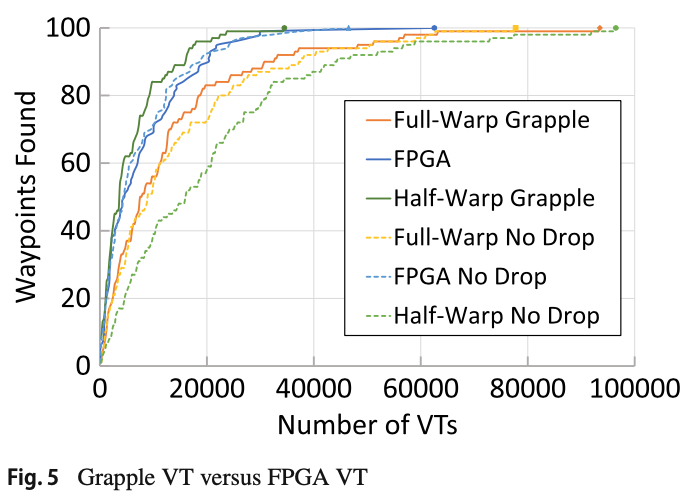
\includegraphics[width=\textwidth]{../evaluation/assets/EXP-00-grapple-paper-waypoints.png}
        \subcaption{Results from the paper. We are only interested in \emph{Full-Warp Grapple}}
        \label{fig:evaluation:EXP-00:1}
    \end{subfigure}
    \begin{subfigure}[b]{.5\textwidth}
        \centering
        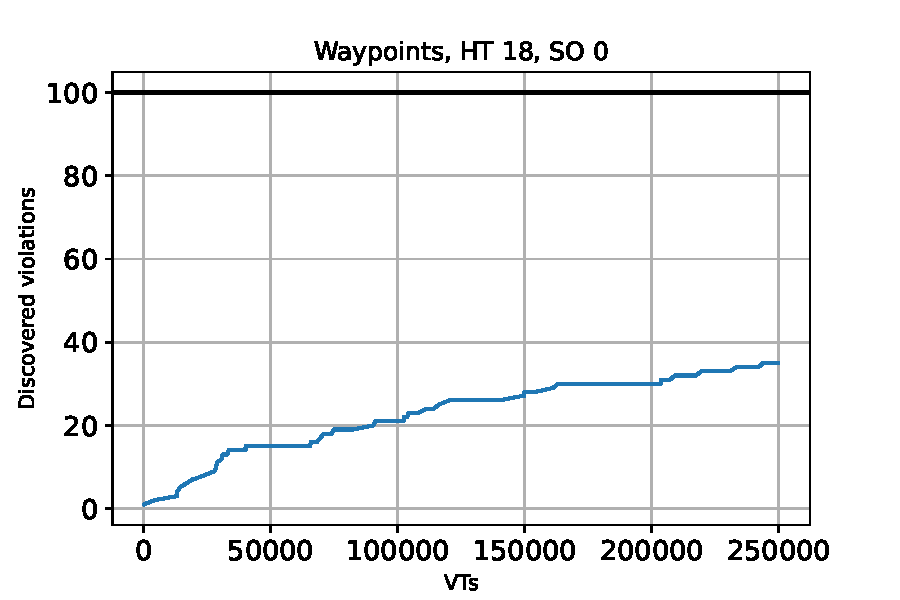
\includegraphics[width=\textwidth]{../evaluation/output-assets/EXP-00-comparison-with-paper.pdf}
        \subcaption{Results of our implementation}
        \label{fig:evaluation:EXP-00:2}
    \end{subfigure}
    \caption{Waypoints model, comparison between reference and our implementation}
    \label{fig:evaluation:EXP-00}
\end{figure}

\subsection{Comparison of Waypoints and HLL as Estimators of State Space Coverage}

As explained in \cref{section:theory:waypoints-model}, counting waypoints is a method for estimating the achieved state space coverage.
To make sure that the discovered waypoints of our implementation correctly indicate the state space coverage, we compare them to the state space coverage estimation of the HyperLogLog introduced in \cref{section:theory:counting-unique-states-visited}.
We would expect both estimators to show similar results.
For example, when 20 waypoints are discovered, the HyperLogLog estimation should show about 20\% state space coverage.

In \cref{fig:evaluation:EXP-01}, results for both estimators are presented.
Clearly, both resemble each other closely.
Thus, we assume them to work correct.
This also confirms the results from our first experiment, underlining our implementation's deficient state space exploration.

\begin{figure}[h]
    \begin{subfigure}[b]{.5\textwidth}
        \centering
        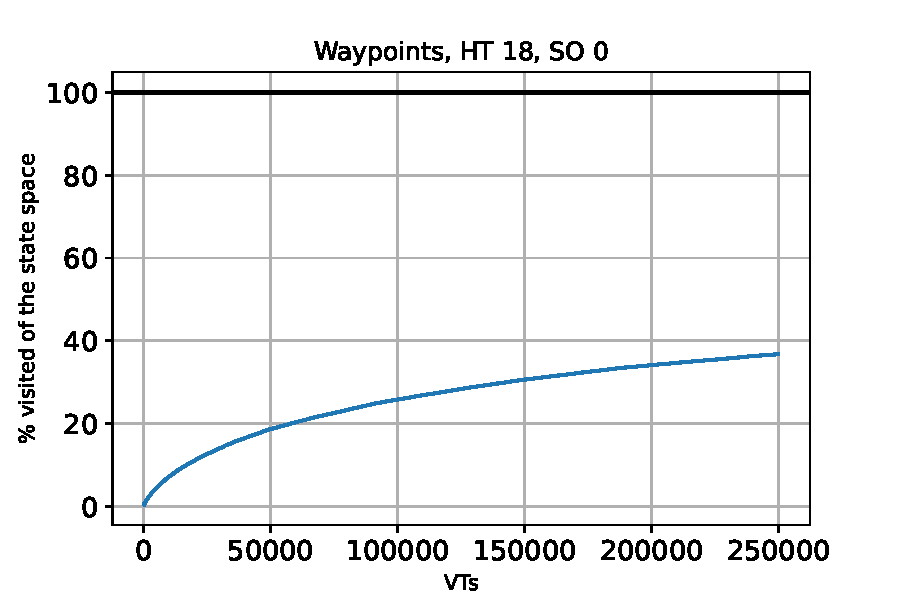
\includegraphics[width=\textwidth]{../evaluation/output-assets/EXP-01-comparison-waypoints-hll-1.pdf}
        \subcaption{HLL state space coverage estimation}
        \label{fig:evaluation:EXP-01:1}
    \end{subfigure}
    \begin{subfigure}[b]{.5\textwidth}
        \centering
        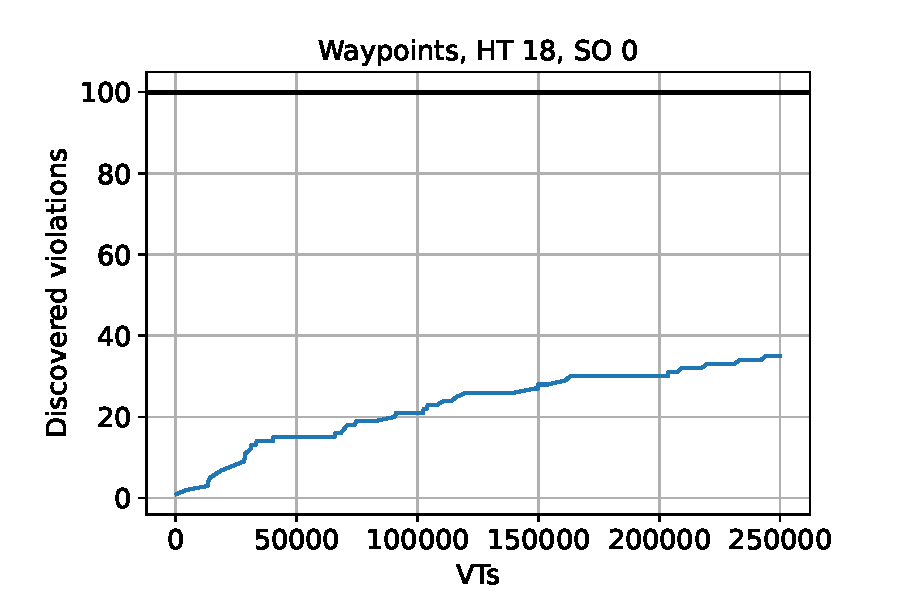
\includegraphics[width=\textwidth]{../evaluation/output-assets/EXP-01-comparison-waypoints-hll-2.pdf}
        \subcaption{Waypoints state space coverage estimation}
        \label{fig:evaluation:EXP-01:2}
    \end{subfigure}
    \caption{Comparison between Waypoints and HyperLogLog state space coverage estimation}
    \label{fig:evaluation:EXP-01}
\end{figure}

\subsection{Impact of Hash Table Size and Sequential VT Execution}

We've identified two key differences of our implementation:
\begin{enumerate}
    \item Our hash tables are 33\% smaller than in the paper.
          This is due to our bit shift implementation presented in \cref{section:implementation:hash-tables} which cannot address the full 48 KB of shared memory.
    \item We batch VTs in a CUDA kernel, each executing 250 at once.
          In the paper, there seems to be only a single VT per CUDA kernel.
\end{enumerate}

To find out whether increasing the hash table size to full 48 KB increases waypoint discovery such that it is similar to the results from the Grapple paper, we've experimentally changed our implementation's addressing.
As the hash table capacity should significantly affect the state space coverage of each VT, we would assume results close to those from the paper.
For each experiment, we've executed 80 runs à 250 VTs (= \num{20000} VTs in total).
Results are shown in \cref{table:EXP-02}.

The larger hash table yields 2.1x as much state space coverage at only 1.45x as many total states visited.
Thus, a larger hash table seems beneficial on this particular model.

However, in the paper, a Grapple swarm verification with \num{392800} hash table slots per VT after \num{20000} VTs discovered 85 waypoints, equalling 85\% state space coverage, which is about 3.7x as much as our large-size hash table implementation.
Resulting from this, the large-size hash table is still far from reproducing the paper's results.

\begin{table}[h]
    \caption{Comparison of different hash table capacities after 80 runs à 250 VTs on the waypoints model}
    \label{table:EXP-02}
    \centering
    \begin{tabular}{l l l l}
        \toprule
        HT Capacity  & State Space Coverage & Total States Visited \\
        \midrule
        \num{262144} & 11.04\%              & \num{63568607}       \\
        \num{393056} & 23.14\%              & \num{91937680}       \\
        \bottomrule
    \end{tabular}
\end{table}

% TODO EXP-03

\section{Low-Connectivity Model Evaluation}
\label{section:evaluation:low-connectivity-model-evaluation}

\section{Validating our implementation and reproducing results from the paper}

We start the evaluation with executing the Waypoints model introduced in \cref{alg:waypoints-model}.
Here, our model checker only implements a parallel BFS with state pruning using hash collisions.
No other diversification techniques are applied.

The results of this first experiment are visualized in \cref{fig:experiments:output1}.
Both sides of the figure visualize the covered state space in relation to the executed VTs.
On the left side, discovered waypoints are used as indicator.
On the right side, the absolute count of the HLL divided by the total state space size is used.

The first observation that can be drawn is, that both indicators are nearly identical.
Having two indicators of state space coverage, we achieve high plausibility that both the waypoints as indicators of state space coverage and the HLL as actual counting of unique visited states operate as intended.

Another observation is that even though \num{250000} VTs are executed, we only cover 35\% of the state space.
This is far below the results from \cite{DeFrancisco2020.Grapple}, where all 100 waypoints are reached after about \num{100000} VTs.

\begin{figure}[h]
    \begin{subfigure}[b]{.5\textwidth}
        \centering
        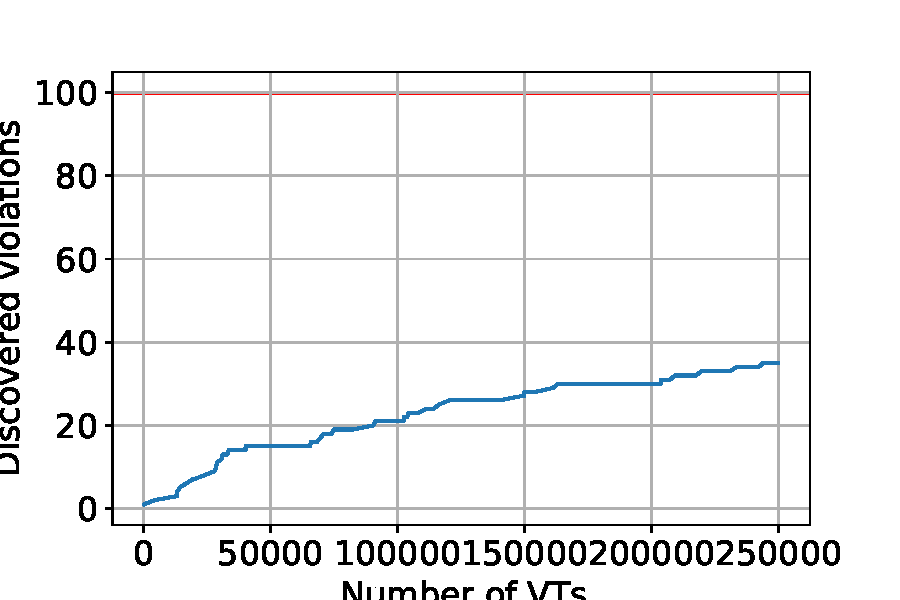
\includegraphics[width=\textwidth]{figures/experiments/output1-discovered-violations-abs-numbers.pdf}
        \subcaption{Discovered violations, absolute numbers}
    \end{subfigure}
    \begin{subfigure}[b]{.5\textwidth}
        \centering
        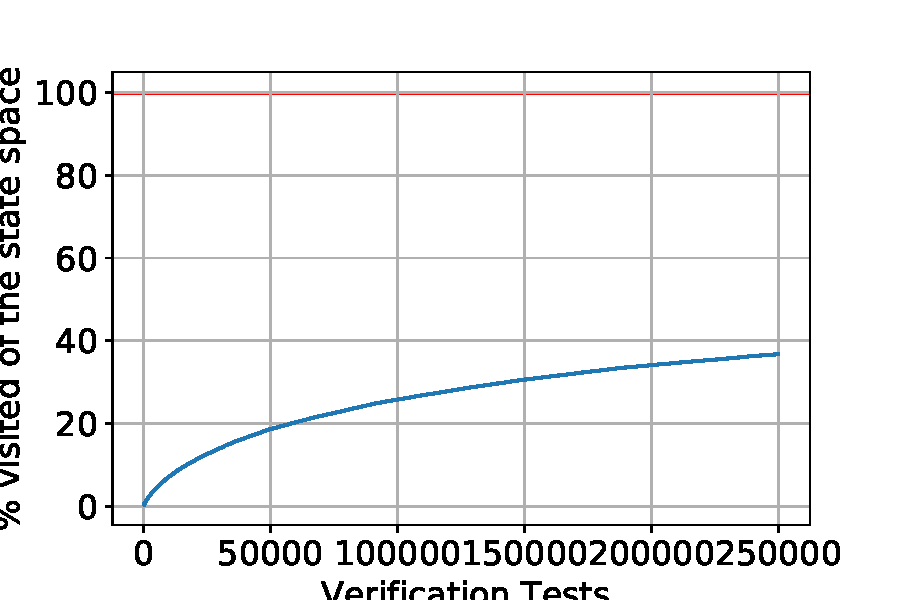
\includegraphics[width=\textwidth]{figures/experiments/output1-covered-state-space-in-percent.pdf}
        \subcaption{Covered state space, in percent}
    \end{subfigure}
    \caption{Waypoints model, \num{1000} runs, $2^{18}$ hash table size, 0 start overs}
    \label{fig:experiments:output1}
\end{figure}

There are two main implementation differences that we believe could lead to the results:

In the paper, hash tables are used that can store nearly \num{400000} entries.
Our hash table can only store \num{262144} entries.
This means that approximately $\frac{1}{3}$ fewer states can be explored per VT, resulting in less depth.
The size of our hash table cannot simply be increased, even though there is shared memory left, as our bit shift based hash bucket addressing only supports table sizes that are an exponent of two.

Another reason may be that in the paper, the number of VTs per run/warp/\dots may be different:
Initially, the paper states that they run \enquote{a single, internally parallel VT per warp}.
Then, however, they state that each CUDA program \enquote{initializes a number of VTs, in this case 250}.
When taking a look at the number of runs in relation to the number of discovered waypoints, results are similar to the paper again.

% - Does it find all waypoints?
% - Does the number of discovered waypoints represent the percentage of covered state space?
% - Is the counted percentage of visited state space plausible?

\section{Introducing Start Overs}

Two key observations are that the state space exploration terminates when the hash table is full and that the rate of hash table collisions and, by that, the number of states that can be visited in a VT is mainly controlled by the hash table size.
This lead to the idea of \emph{start overs}, which is based on the two-phase swarm of \cite{DeFrancisco2020.Grapple}.
After a VT considers itself done,

\begin{figure}[h]
    \centering
    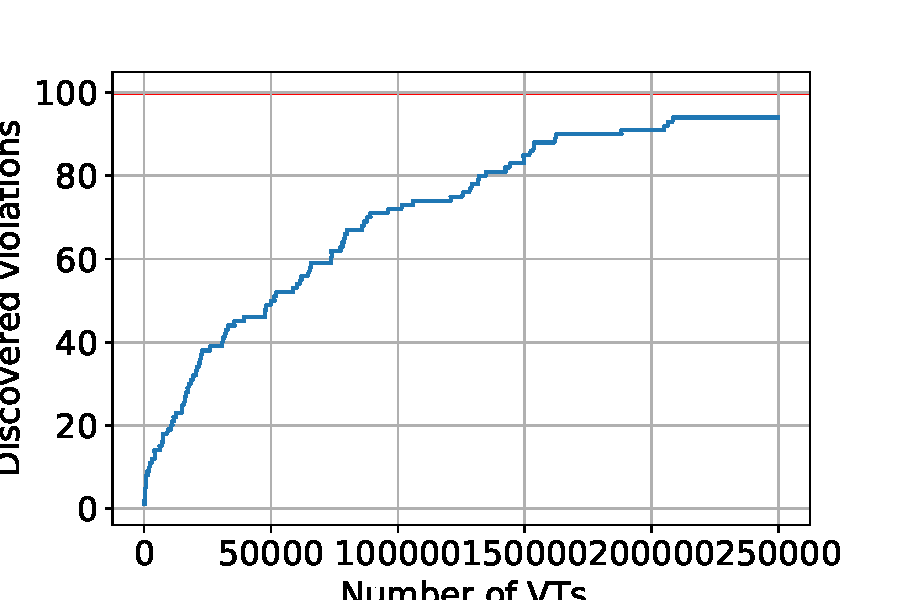
\includegraphics[width=.5\textwidth]{figures/experiments/output2-discovered-violations-abs-numbers.pdf}
    \caption{Waypoints model, \num{1000} runs, $2^{14}$ hash table size, 15 start overs}
    \label{fig:experiments:output2}
\end{figure}

% Philosophers ?? Anderson ??

\section{Low-Connectivity Models}

The Grapple paper suspects two models of being low-connectivity:
Andersons queue lock mutual exclusion algorithm and the Dining Philosophers Problem.
Both models are taken from the BEEM database. % TODO add citation to BEEM db

The difference in model checking performance between the \emph{high-connectivity} Waypoints model and the \emph{low-connectivity} Anderson and Philosophers models can be observed by comparing the number of unique states visited of the models using the same model checker configuration.
\cref{table:lc-comparison} contains results for the three models.

\begin{table}[h]
    \caption{Comparison of three models, executed with 250 VTs (one run), $2^{14}$ hash table size and 10 start overs}
    \label{table:lc-comparison}
    \centering
    \begin{tabular}{l l l l}
        \toprule
        Model          & Unique States Visited & Total States Visited & Covered State Space \\
        \midrule
        Anderson 3     & \num{284941}          & \num{26688449}       & -                   \\
        Philosopher 15 & \num{7.87901e+06}     & \num{44674703}       & ~55\%               \\
        Waypoints      & \num{3.18306e+07}     & \num{45032805}       & ~0.74\%             \\
        \bottomrule
    \end{tabular}
\end{table}

\section{Optimizing Grapple on Low-Connectivity Models}

% How can the algorithm be altered so that it can efficiently search low-connectivity models?
%% Precondition: We only consider models with >100% hash table utilization. Models with less utilization are checked exhaustively either way.
%% Goal: Maximize state space coverage while minimizing the amount of VTs required to do so.
%% Benchmark 1: Comparison with the baseline implementation.
%% ? Benchmark 2: Comparison with the Waypoints model (how?) ?

\chapter{Conclusion}

\section{Future work}

- Estimate state space size for models of unknown size
- Automatically determine the optimal number of start overs
- Implement usage of multiple GPU devices through CUDA streaming API
- Analyze State Space Diversification, i.e. "how good is a partition?"

\section{Discussion}

% \appendix

% \chapter{Listings}

\backmatter

\printbibliography[heading=bibintoc]

\end{document}
